% !TEX root=../main.tex

\section{Properties}
\label{sec:properties}

We define an evaluation function that takes a task, state and list of inputs,
and returns the value of the task after application of all inputs.
This is a partial function since not all tasks have an observable value.

\begin{figure*}[t]
  \begin{function}
    \signature{\Evaluate : \mathrm{Tasks} \times \mathrm{States} \times [\mathrm{Inputs}]
      \rightarrow \mathrm{Values}} \\
    \Evaluate\ (t,\sigma,[])       &=& \Value(t,\sigma)\\
    \Evaluate\ (t, \sigma, (i:is)) &=& \left\{
      \begin{array}{lr}
        v                                                                                 & \Value(t,\sigma)=v\\
        \Evaluate\ (t',\sigma',is)                                                                &  \Value(t,\sigma)=\bot \land t,\sigma\xRightarrow[]{i}t',\sigma'
      \end{array}
    \right.
  \end{function}
  \caption{evaluate function definition.}
  \label{fig:evaluate}
\end{figure*}

All elements of firsts are valid hints.

\begin{definition}[$t,\sigma\drive{I}^* v$]
  \begin{align*}
    t,\sigma             & \drive{i_1} & t_1,\sigma_1\\
    t_1,\sigma_1         & \drive{i_2} & t_2,\sigma_2\\
                         & \vdots   & \\
    t_{n-1},\sigma_{n-1} & \drive{i_n} & t_n,\sigma_n
  \end{align*}
  With $\Value(t_n,\sigma_n)=v$\\
  $\Value(t_{i<n},\sigma_{i<n})=\bot$\\
  $I=i_1,\cdots,i_n$
\end{definition}

\subsection{Correctness of firsts}

The most important property we would like to prove, is the correctness of the hints calculated by firsts.
Intuitively, for a set of next step hints to be correct, they should be
- valid steps a user can actually take
- bring the user closer to the desired goal
- contain ALL steps that bring the user closer to their goal.

We separate this property into two parts.


\begin{lemma}[Soundness of firsts]
  \label{lem:soundfirsts}

  % For all tasks $t$, states $\sigma$ and goals $g$,
  % such that for all $(\tilde{i},\phi)\in firsts\ (\tilde{t},\tilde{\sigma},g)$,
  % there exists a mappings $M = [s_0\mapsto c_0,\cdots,s_n\mapsto c_n]$
  % such that $t,M \sigma \xRightarrow[]{M i} t',\sigma'$.
  % Subsequently, there exists a sequence of inputs $I$ such that $\Evaluate (t',\sigma',I) = v$
  % with $g v = \True$.
  % \todo{strictly speaking, this allows for empty/bogus hints that do not get CLOSER to the goal.}
\end{lemma}


\begin{lemma}[Completeness of firsts]
  \label{lem:completefirsts}
  %
  % For all tasks $t$, states $\sigma$, lists of inputs $(i:is)$ and goals $g$,
  % such that $\Evaluate\ (t,\sigma,(i:is))=v$ with $g\ v =\True$,
  % then $i\in firsts\ (t,\sigma,g)$.

\end{lemma}


Since the $\Firsts$ function relies on the $\Simulate$ function, we can make use of soundness and completeness of that function with respect to $\Evaluate$, when proving the lemma's above.

\begin{lemma}[Soundness of simulate]
  \label{lem:soundsimulate}
  For all tasks $t$ and states $\sigma$
  such that $t,\sigma\drive{}^*\overline{\tilde{v},\tilde{I},\Phi}$
  then for all results $(\tilde{v},\tilde{I}=[\tilde{i}_0,\cdots,\tilde{i}_n],\Phi)$
  there exists a concrete input $I$ with the same length as the symbolic input $\tilde{I}$
  such that $t,\sigma\drive{I}^*v$
  with $[s_i\mapsto c_i]\tilde{v}=v$ and $[s_i\mapsto c_i]\Phi$
  where $s_i\in\tilde{i_i}$ and $c_i\in i_i$.
\end{lemma}

\begin{lemma}[Completeness of simulate]
  \label{lem:completesimulate}
  For all tasks $t$, states $\sigma$ and lists of input $I$
  such that $t,\sigma\drive{I}^*v$
  there exists a symbolic value $\tilde{v}$ and a symbolic input $\tilde{I}$ with the same length as $I$,
  such that $(\tilde{v},\tilde{I},\Phi)\in t,\sigma\drive{}^*$,
  with $\tilde{i_i}\sim i_i$, $[s_i\mapsto c_i]\tilde{v}=v$ and $[s_i\mapsto c_i]\Phi$,
  where $s_i\in\tilde{i_i}$ and $c_i\in i_i$.
\end{lemma}


$\Evaluate$ and $\Simulate$ make use of the driving and symbolic driving semantics respectively, so we again first prove those sound and complete with respect to each other.

\begin{lemma}[Soundness of driving]
  \label{lem:sounddriving}
  For all tasks $t$ and states $\sigma$,
  if $t,\sigma\drive{} \overline{\tilde{t},\tilde{\sigma},\tilde{i},\phi}$
  then for all tuples $(\tilde{t},\tilde{\sigma},\tilde{i},\phi)$,
  there exists an $i$ such that
  $t,\sigma\drive{i}t',\sigma'$
  with $\tilde{i}\sim i$, $[s\mapsto c]\tilde{t}=t'$ and $[s\mapsto c]\tilde{\sigma}=\sigma'$ where $s\in \tilde{i}$ and $c\in i$.
\end{lemma}

\begin{lemma}[Completeness of driving]
  \label{lem:completedriving}
  For all tasks $t$, states $\sigma$ and inputs $i$,
  if $t,\sigma\drive{i}t',\sigma'$,
  then there exists an $\tilde{i}\sim i$, $\tilde{t}$ and $\tilde{\sigma}$
  such that $t,\sigma\drive{}\tilde{t},\tilde{\sigma},\tilde{i},\phi$
  with $[s\mapsto c]\tilde{t}=t'$, $[s\mapsto c]\tilde{\sigma}=\sigma'$ and $[s\mapsto c]\phi$, where $s\in \tilde{i}$ and $c\in i$.
\end{lemma}

Where $\tilde{i}\sim i$ is defined as follows.

\begin{definition}[Input simulation]
  A symbolic input $\tilde{i}$ simulates a concrete input $i$ denoted as $\tilde{i}\sim i$ in the following cases.\\
  $s\sim a$, where $s$ is a symbol and $a$ a concrete action.\\
  $\tilde{i}\sim i\implies \First \tilde{i} \sim \First i$\\
  $\tilde{i}\sim i\implies \Second \tilde{i} \sim \Second i$
\end{definition}

And $s\in \tilde{i}$ and $c\in i$ are defined as follows.

\begin{definition}[Value from input]
  $c\in \First i = c\in i $\\
  $c\in \Second i = c\in i $\\
  $c\in a = a $
\end{definition}

\begin{definition}[Symbol from input]
  $s\in \First \tilde{i} = s\in \tilde{i} $\\
  $s\in \Second \tilde{i} = s\in \tilde{i} $\\
  $s\in a = a $
\end{definition}

Since the driving semantics depends on the handling and normalisation semantics, we need to show that they too are sound and complete, before we can prove the lemma's above.


\begin{lemma}[Soundness of handling]
  \label{lem:soundhandle}

  For all tasks $t$ and states $\sigma$,
  if $t,\sigma\handle{}\overline{\tilde{t'},\tilde{\sigma'},\tilde{i},\phi}$
  then for all tuples $(\tilde{t'},\tilde{\sigma'},\tilde{i}\phi)$
  there exists an input $i$ such that $t,\sigma\handle{i}t',\sigma'$
  with $\tilde{i}\sim i$, $[s\mapsto c]\tilde{t}=t'$ and $[s\mapsto c]\tilde{\sigma}=\sigma'$ where $s\in \tilde{i}$ and $c\in i$.
  
\end{lemma}

\begin{lemma}[Soundness of normalisation]
  \label{lem:soundnorm}

  For all expressions $e$, states $\sigma$ and mappings $M=[s_0\mapsto c_0,\cdots,s_n\mapsto c_n]$,
  such that $e,\sigma\normalise \overline{t,\sigma',\phi}$,
  we have $M\phi$ implies
  $e,M \sigma \hat{\normalise}t',\sigma''$, $t M \equiv t'$ and $\sigma' M \equiv \sigma''$.
\end{lemma}

\begin{lemma}[Soundness of striding]
  For all tasks $t$, states $\sigma$ and mappings $M=[s_0\mapsto c_0,\cdots,s_n\mapsto c_n]$,
such that $t,\sigma\stride \overline{t',\sigma',\phi}$,
$M \phi$ implies
$t,M\sigma \hat{\stride}\bar{t'},\bar{\sigma'}$, $M t'\ \equiv \bar{t'} \land M\sigma' \equiv \bar{\sigma'}$.
\end{lemma}

\begin{lemma}[Soundness of evaluation]
  For all expressions $e$, states $\sigma$ and mappings $M=[s_0\mapsto c_0,\cdots,s_n\mapsto c_n]$,
such that $e,\sigma\eval \overline{v,\sigma',\phi}$,
we have that $M\phi$ implies
$t,M\sigma \hat{\eval}\bar{v},\bar{\sigma'} \land Mv \equiv \bar{v} \wedge M\sigma' \equiv \bar{\sigma'}$.
\end{lemma}

\begin{lemma}[Completeness of handling]
  \label{lem:completeHandle}
    For all $t,\sigma,j$ such that $t,\sigma \xrightarrow[]{j} \hat{t'},\hat{\sigma'}$
    there exists an $i\sim j$ such that $t,\sigma''\handle{} t'',\sigma''',i,\phi$.
\end{lemma}

\begin{lemma}[Completeness of normalisation]
  \label{lem:completeNormalise}
  For all $e,\sigma$ such that $e,\sigma \hat{\normalise}\hat{t},\hat{\sigma}$
  there exists a symbolic execution $e,\sigma\normalise \hat{t},\hat{\sigma},\True$.
\end{lemma}

\begin{lemma}[Completeness of striding]
  \label{lem:completeStride}
  For all $t,\sigma$ such that $t,\sigma \hat{\stride}\hat{t},\hat{\sigma}$
  there exists a symbolic execution $t,\sigma\eval \hat{t},\hat{\sigma},\True$.
\end{lemma}

\begin{lemma}[Completeness of evaluate]
  \label{lem:completeEval}
    For all $e,\sigma$ such that $e,\sigma \hat{\eval}\hat{v},\hat{\sigma}$
    there exists a symbolic execution $e,\sigma\eval \hat{v},\hat{\sigma},\True$.
\end{lemma}

The problem with the lemma's above, is that they assume that you start out with the same task and state.
In the case of $\Evaluate$ and $\Simulate$, this is not true, since in the sequential application of (symbolic) drive, the expressions differ.
Below, a graphical representation is shown of this process.

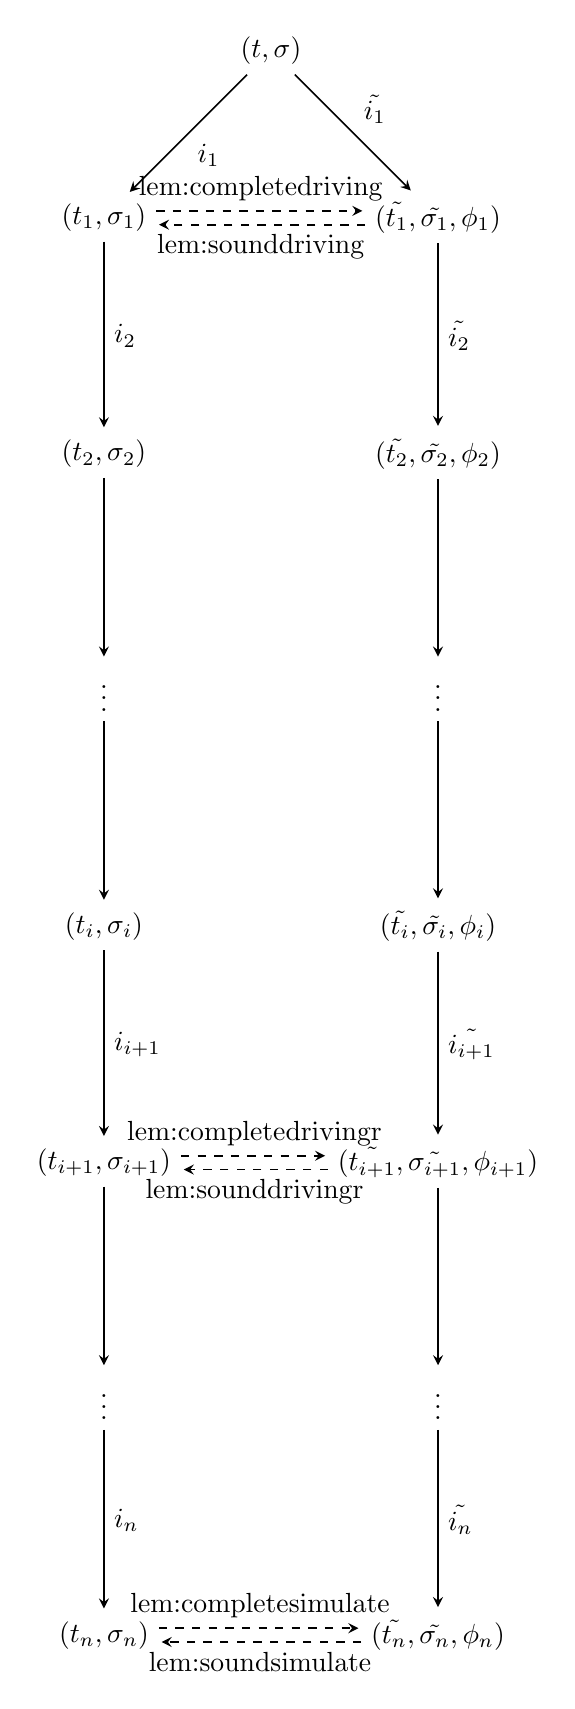
\begin{tikzpicture}[
            > = stealth, % arrow head style
            shorten > = 1pt, % don't touch arrow head to node
            auto,
            node distance = 3cm, % distance between nodes
            semithick % line style
        ]



        \node (0) {$(t,\sigma)$};
        \node (c1) [below left of=0] {$(t_1,\sigma_1)$};
        \node (s1) [below right of=0] {$(\tilde{t_1},\tilde{\sigma_1},\phi_1)$};
        \node (c2) [below of=c1] {$(t_2,\sigma_2)$};
        \node (s2) [below of=s1] {$(\tilde{t_2},\tilde{\sigma_2},\phi_2)$};
        \node (ccc) [below of=c2] {\vdots};
        \node (sss) [below of=s2] {\vdots};
        \node (ci) [below of=ccc] {$(t_i,\sigma_i)$};
        \node (si) [below of=sss] {$(\tilde{t_i},\tilde{\sigma_i},\phi_i)$};
        \node (cii) [below of=ci] {$(t_{i+1},\sigma_{i+1})$};
        \node (sii) [below of=si] {$(\tilde{t_{i+1}},\tilde{\sigma_{i+1}},\phi_{i+1})$};
        \node (cc) [below of=cii] {\vdots};
        \node (ss) [below of=sii] {\vdots};
        \node (cn) [below of=cc] {$(t_n,\sigma_n)$};
        \node (sn) [below of=ss] {$(\tilde{t_n},\tilde{\sigma_n},\phi_n)$};

        \path[->] (0) edge node {$i_1$} (c1);
        \path[->] (0) edge node {$\tilde{i_1}$} (s1);
        \path[->] (c1) edge node {$i_2$} (c2);
        \path[->] (s1) edge node {$\tilde{i_2}$} (s2);
        \path[->] (c2) edge node { } (ccc);
        \path[->] (s2) edge node { } (sss);
        \path[->] (ccc) edge node { } (ci);
        \path[->] (sss) edge node { } (si);
        \path[->] (ci) edge node {$i_{i+1}$} (cii);
        \path[->] (si) edge node {$\tilde{i_{i+1}}$} (sii);
        \path[->] (cii) edge node { } (cc);
        \path[->] (sii) edge node { } (ss);
        \path[->] (cc) edge node {$i_n$} (cn);
        \path[->] (ss) edge node {$\tilde{i_n}$} (sn);

        \path[dashed,->] ([yshift=.25em]c1.east) edge node {\cref{lem:completedriving}} ([yshift=.25em]s1.west);
        \path[dashed,->] ([yshift=-.25em]s1.west) edge node {\cref{lem:sounddriving}} ([yshift=-.25em]c1.east);

        \path[dashed,->] ([yshift=.25em]cii.east) edge node {\cref{lem:completedrivingr}} ([yshift=.25em]sii.west);
        \path[dashed,->] ([yshift=-.25em]sii.west) edge node {\cref{lem:sounddrivingr}} ([yshift=-.25em]cii.east);

        \path[dashed,->] ([yshift=.25em]cn.east) edge node {\cref{lem:completesimulate}} ([yshift=.25em]sn.west);
        \path[dashed,->] ([yshift=-.25em]sn.west) edge node {\cref{lem:soundsimulate}} ([yshift=-.25em]cn.east);

    \end{tikzpicture}

to be added to the figure above:\\
$\Value(t_n,\sigma_n)=v$\\
$\Value(t_{i<n},\sigma_{i<n})=\bot$\\
etc

\begin{definition}[Consistance relation $R$]
$R(t,\sigma,\tilde{t},\tilde{\sigma},\Phi)
\iff\exists M . M\tilde{t}=t
\land M\tilde{\sigma}=\sigma
\land M\Phi$
With $M$ the minimal substitution $[s_1\mapsto c_1,\cdots,s_n\,mapsto c_n]$. (ie no symbols in $M$ that are not present in $\tilde{t}$)
\end{definition}

\begin{lemma}[Soundness of driving with respect to $R$]
  \label{lem:sounddrivingr}
$R(t,\sigma,\tilde{t},\tilde{\sigma},\Phi)$ implies
that for all symbolic inputs $\tilde{i}$ such that $\tilde{t},\tilde{\sigma}\drive{}\overline{\tilde{t}',\tilde{\sigma}',\tilde{i},\phi}$ and $\Sat(\Phi\land\phi)$,
there exists an input $i$ such that $t,\sigma\drive{i}t',\sigma'$ and $R(t',\sigma',\tilde{t}',\tilde{\sigma}',\Phi\land\phi)$


\end{lemma}

\begin{lemma}[Completeness of driving with respect to $R$]
  \label{lem:completedrivingr}
  $R(t,\sigma,\tilde{t},\tilde{\sigma},\Phi)$ implies
  that for all inputs $i$ such that $t,\sigma\drive{i}t',\sigma'$,
  there exists a symbolic input $\tilde{i}$ such that $\tilde{t},\tilde{\sigma}\drive{}\overline{\tilde{t}',\tilde{\sigma}',\tilde{i},\phi}$, $\Sat(\Phi\land\phi)$ and $R(t',\sigma',\tilde{t}',\tilde{\sigma}',\Phi\land\phi)$.
\end{lemma}
